\documentclass[11pt,letterpaper]{article}

\usepackage[top=0.82in,bottom=0.72in,left=0.92in,right=0.92in]{geometry}
\usepackage{amsmath,amssymb,mathtools}
\usepackage{array,booktabs,tabularx,multirow}
\usepackage{enumitem}
\usepackage{xcolor}
\usepackage{tikz}
\usetikzlibrary{arrows.meta,positioning}
\usepackage{pgfplots}
\pgfplotsset{compat=1.18}
\usepackage{fancyhdr}
\usepackage{microtype}

\setlength{\parindent}{0pt}
\setlength{\parskip}{0.42em}
\setlength{\headheight}{13.6pt}
\setlength{\footskip}{0.38in}
\setlist[enumerate]{itemsep=0.28em,topsep=0.3em}

\pagestyle{fancy}
\fancyhf{}
\fancyfoot[C]{Page \thepage\ of \pageref{LastPage}}
\renewcommand{\headrulewidth}{0pt}
\renewcommand{\footrulewidth}{0pt}

\fancypagestyle{lastpage}{%
  \fancyhf{}
  \fancyfoot[C]{Page \thepage\ of \pageref{LastPage}}
  \fancyfoot[R]{End of exam}
  \renewcommand{\headrulewidth}{0pt}
  \renewcommand{\footrulewidth}{0pt}
}

\newenvironment{examquestion}[2]{%
  \clearpage
  \begin{list}{}{%
    \setlength{\leftmargin}{2.15em}%
    \setlength{\labelwidth}{1.55em}%
    \setlength{\labelsep}{0.60em}%
    \setlength{\itemindent}{0pt}%
    \setlength{\listparindent}{0pt}%
    \setlength{\parsep}{0.42em}%
    \setlength{\topsep}{0pt}%
  }
  \item[\hfill #1.] (#2 points)\ 
}{%
  \end{list}
}

\newenvironment{solution}{%
  \par\medskip
  \color{red}
  \noindent\textbf{Solution.}\par
}{%
  \par
  \color{black}
}

\newcommand{\E}{\mathbb{E}}
\newcommand{\Prob}{\mathbb{P}}
\newcommand{\R}{\mathbb{R}}
\newcommand{\answerbox}[1]{%
  \par\smallskip\begingroup
  \setlength{\fboxsep}{4pt}%
  \setlength{\fboxrule}{0.7pt}%
  \noindent\makebox[\linewidth][c]{\fbox{$\displaystyle #1$}}%
  \par\endgroup\smallskip
}
\newcommand{\answerboxtext}[1]{%
  \par\smallskip\begingroup
  \setlength{\fboxsep}{4pt}%
  \setlength{\fboxrule}{0.7pt}%
  \noindent\makebox[\linewidth][c]{%
    \fbox{\parbox{0.84\linewidth}{\centering #1}}}%
  \par\endgroup\smallskip
}

\begin{document}

\thispagestyle{empty}

\begin{center}
  \vspace*{0.30in}
  {\LARGE The Hong Kong University of Science and Technology}\par
  \vspace{0.12em}
  {\LARGE IEDA 1250, Summer 2026}\par
  \vspace{0.12em}
  {\LARGE Final Exam \textcolor{red}{Solution}}\par
\end{center}

\vspace{0.28in}

\noindent
\begin{tabularx}{\textwidth}{@{}X X@{}}
Student ID\ \rule{1.55in}{0.4pt} & \hfill Name:\ \rule{2.65in}{0.4pt}
\end{tabularx}

\vspace{0.30in}

\begingroup
\setlength{\fboxsep}{4pt}
\begin{center}
\fbox{\fbox{%
\begin{minipage}{0.86\textwidth}
\vspace{0.10in}
\begin{center}
\textbf{\large Please read the following instructions carefully.}
\end{center}
\begin{itemize}[leftmargin=2.0em,itemsep=0.65em]
  \item You have \textbf{120} minutes to complete this exam. This question booklet
  contains \textbf{7} questions for a total of 120 points. Check to see if any pages
  are missing.
  \item Read the instructions for individual questions carefully before answering
  the questions.
  \item \textbf{Please write your answers in the answer book.} You can use this
  question booklet as scratch paper.
\end{itemize}
\vspace{0.08in}
\end{minipage}%
}}
\end{center}
\endgroup

\vspace{0.27in}

\begin{center}
\renewcommand{\arraystretch}{1.68}
\begin{tabular}{|c|c|c|}
\hline
Question & Points & Score\\ \hline
1 & 20 & \\ \hline
2 & 20 & \\ \hline
3 & 20 & \\ \hline
4 & 20 & \\ \hline
5 & 20 & \\ \hline
6 & 10 & \\ \hline
7 & 10 & \\ \hline
Total & 120 & \\ \hline
\end{tabular}
\end{center}

% -----------------------------------------------------------------------------
\begin{examquestion}{1}{20}
Consider the zero-sum game having the following payoff table for Player 1:

\begin{center}
\begin{tabular}{cc|cc}
&&\multicolumn{2}{c}{\textbf{Player 2}}\\
&&$S_1$&$S_2$\\ \cline{2-4}
\multirow{2}{*}{\textbf{Player 1}}&$S_1$&3&$-2$\\
&$S_2$&$-1$&2\\ \cline{2-4}
\end{tabular}
\end{center}

\begin{enumerate}[label=(\alph*),leftmargin=2.2em]
  \item Use the graphical procedure to determine the value of the game and the
  optimal mixed strategy for each player.
  \item Check your answer by (i) constructing Player 2's payoff table and
  (ii) applying the graphical procedure again to the resulting table.
\end{enumerate}

\begin{solution}
\textbf{(a)} Let Player 1 choose $S_1$ with probability $x$ and $S_2$ with
probability $1-x$. If Player 2 chooses $S_1$ or $S_2$, respectively, Player 1's
expected payoff is
\[
L_1(x)=3x-(1-x)=4x-1,
\qquad
L_2(x)=-2x+2(1-x)=2-4x.
\]
Player 1 maximizes the lower envelope of these two lines. Graphically, the maximum
occurs at their intersection:
\[
4x-1=2-4x
\quad\Longrightarrow\quad
x=\frac38,
\qquad
v=\frac12.
\]

\begin{center}
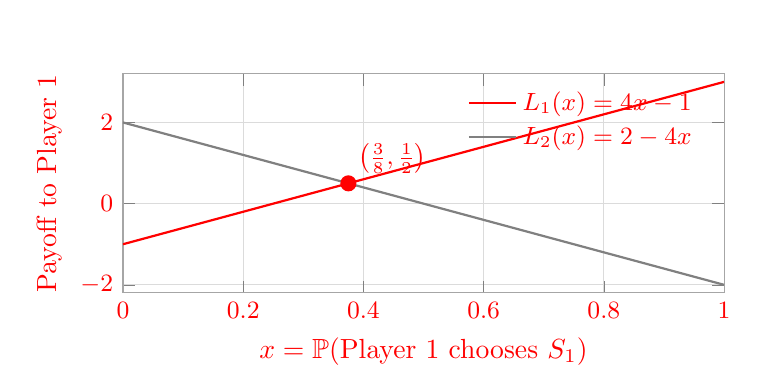
\begin{tikzpicture}
\begin{axis}[
  width=0.76\textwidth,
  height=0.36\textwidth,
  xmin=0,xmax=1,
  ymin=-2.2,ymax=3.2,
  xlabel={$x=\Prob(\text{Player 1 chooses }S_1)$},
  ylabel={Payoff to Player 1},
  grid=both,
  major grid style={gray!28},
  axis line style={gray!70},
  tick label style={font=\small,color=red},
  label style={color=red},
  legend style={draw=none,fill=none,font=\small,text=red},
  legend pos=north east
]
  \addplot[red,thick,domain=0:1,samples=2]{4*x-1};
  \addlegendentry{$L_1(x)=4x-1$}
  \addplot[gray,thick,domain=0:1,samples=2]{2-4*x};
  \addlegendentry{$L_2(x)=2-4x$}
  \addplot[red,only marks,mark=*,mark size=2.7pt]
    coordinates {(0.375,0.5)};
  \node[anchor=south west,text=red,font=\small] at (axis cs:0.375,0.5)
    {$\left(\frac38,\frac12\right)$};
\end{axis}
\end{tikzpicture}
\end{center}

Therefore, Player 1's optimal strategy is
\[
p^*=\left(\frac38,\frac58\right).
\]
Let Player 2 choose $S_1$ with probability $q$. To make Player 1 indifferent
between the two rows,
\[
3q-2(1-q)=-q+2(1-q)
\quad\Longrightarrow\quad
q=\frac12.
\]
Hence Player 2's optimal strategy and the value to Player 1 are
\[
q^*=\left(\frac12,\frac12\right),
\qquad v=\frac12.
\]

\textbf{(b)} Player 2's payoff is the negative of Player 1's payoff. With Player
2's strategies as rows, its payoff table is
\[
\begin{array}{c|cc}
&\text{Player 1 }S_1&\text{Player 1 }S_2\\ \hline
\text{Player 2 }S_1&-3&1\\
\text{Player 2 }S_2&2&-2
\end{array}.
\]
If Player 2 chooses its first row with probability $q$, its payoff against Player
1's two columns is
\[
H_1(q)=-3q+2(1-q)=2-5q,
\qquad
H_2(q)=q-2(1-q)=3q-2.
\]
The lower-envelope maximum satisfies
\[
2-5q=3q-2
\quad\Longrightarrow\quad
q=\frac12,
\qquad
v_2=-\frac12.
\]

\begin{center}
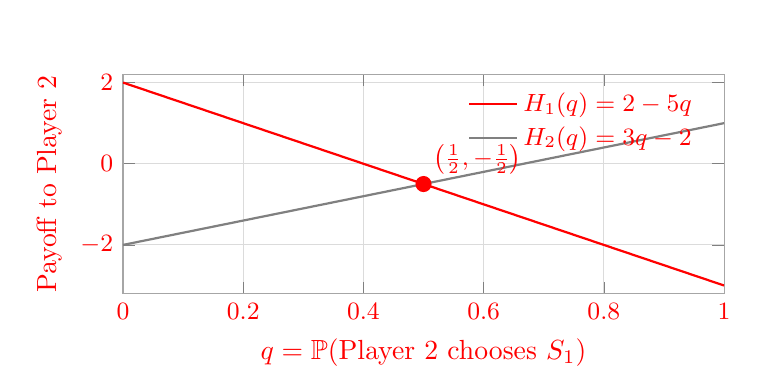
\begin{tikzpicture}
\begin{axis}[
  width=0.76\textwidth,
  height=0.36\textwidth,
  xmin=0,xmax=1,
  ymin=-3.2,ymax=2.2,
  xlabel={$q=\Prob(\text{Player 2 chooses }S_1)$},
  ylabel={Payoff to Player 2},
  grid=both,
  major grid style={gray!28},
  axis line style={gray!70},
  tick label style={font=\small,color=red},
  label style={color=red},
  legend style={draw=none,fill=none,font=\small,text=red},
  legend pos=north east
]
  \addplot[red,thick,domain=0:1,samples=2]{2-5*x};
  \addlegendentry{$H_1(q)=2-5q$}
  \addplot[gray,thick,domain=0:1,samples=2]{3*x-2};
  \addlegendentry{$H_2(q)=3q-2$}
  \addplot[red,only marks,mark=*,mark size=2.7pt]
    coordinates {(0.5,-0.5)};
  \node[anchor=south west,text=red,font=\small] at (axis cs:0.5,-0.5)
    {$\left(\frac12,-\frac12\right)$};
\end{axis}
\end{tikzpicture}
\end{center}

Finally, Player 1 makes Player 2 indifferent between its rows:
\[
-3x+(1-x)=2x-2(1-x)
\quad\Longrightarrow\quad
x=\frac38.
\]
Thus the second graphical calculation confirms
\answerbox{
p^*=\left(\frac38,\frac58\right),
\qquad
q^*=\left(\frac12,\frac12\right),
\qquad
v_1=\frac12,\quad v_2=-\frac12
}
\end{solution}
\end{examquestion}

% -----------------------------------------------------------------------------
\begin{examquestion}{2}{20}
Consider the following zero-sum two-player game. The entries in the table are the
payoffs to Player A.

\begin{center}
\begin{tabular}{c|rrrrrr}
&$B_1$&$B_2$&$B_3$&$B_4$&$B_5$&$B_6$\\ \hline
$A_1$&1&10&2&3&11&12\\
$A_2$&4&8&5&6&9&10\\
$A_3$&7&5&8&9&6&7\\
$A_4$&10&1&11&12&2&3\\
$A_5$&3&7&4&5&8&9\\
$A_6$&6&4&7&8&5&6
\end{tabular}
\end{center}

Player A chooses one of the six rows, and Player B chooses one of the six columns.
Player A wants to maximize the expected payoff, while Player B wants to minimize the
expected payoff.

\begin{enumerate}[label=(\alph*),leftmargin=2.2em]
  \item Find the Nash equilibrium in this game and report the value of the game.
  \item Write Player A's linear program for the \emph{full} payoff table.
  \item The following linear program is associated with Player B. Let $q_j$ be the
  probability that Player B chooses column $j$, for $j=1,\ldots,6$, and let $v_B$
  represent the expected loss of Player B:
  \[
  \begin{aligned}
  \min\quad &v_B\\
  \text{s.t.}\quad
  &q_1+10q_2+2q_3+3q_4+11q_5+12q_6\le v_B,\\
  &4q_1+8q_2+5q_3+6q_4+9q_5+10q_6\le v_B,\\
  &7q_1+5q_2+8q_3+9q_4+6q_5+7q_6\le v_B,\\
  &10q_1+q_2+11q_3+12q_4+2q_5+3q_6\le v_B,\\
  &3q_1+7q_2+4q_3+5q_4+8q_5+9q_6\le v_B,\\
  &6q_1+4q_2+7q_3+8q_4+5q_5+6q_6\le v_B,\\
  &q_1+q_2+q_3+q_4+q_5+q_6=1,\\
  &q_1,q_2,q_3,q_4,q_5,q_6\ge0,\\
  &v_B\text{ is unrestricted in sign.}
  \end{aligned}
  \]
  Show that Player A's LP and Player B's LP are primal and dual LPs. That is,
  starting from Player A's LP in part (b), derive its dual and show that the dual
  is identical to the given one.
\end{enumerate}

\begin{solution}
\textbf{(a)} First eliminate dominated strategies. For Player A, row $A_5$ is
strictly dominated by $A_2$, and row $A_6$ is strictly dominated by $A_3$. For
Player B, columns $B_3$ and $B_4$ are dominated by $B_1$, and columns $B_5$ and
$B_6$ are dominated by $B_2$. The reduced payoff matrix is
\[
\begin{array}{c|cc}
&B_1&B_2\\ \hline
A_1&1&10\\
A_2&4&8\\
A_3&7&5\\
A_4&10&1
\end{array}.
\]

Let $q$ be the probability that Player B chooses $B_1$. The expected payoff to
Player A from each remaining row is
\[
\begin{aligned}
g_1(q)&=10-9q, & g_2(q)&=8-4q,\\
g_3(q)&=5+2q,  & g_4(q)&=1+9q.
\end{aligned}
\]
Player B minimizes the upper envelope. The relevant intersection is between
$g_2$ and $g_3$:
\[
8-4q=5+2q
\quad\Longrightarrow\quad
q=\frac12,
\qquad v=6.
\]

\begin{center}
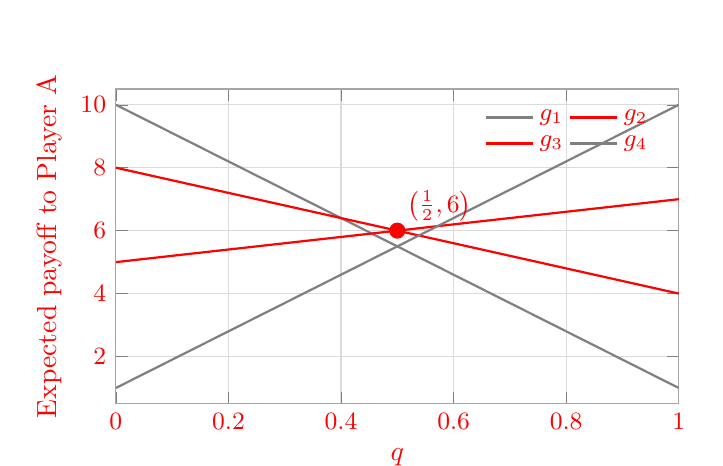
\begin{tikzpicture}
\begin{axis}[
  width=0.72\textwidth,
  height=0.46\textwidth,
  xmin=0,xmax=1,
  ymin=0.5,ymax=10.5,
  xlabel={$q$},ylabel={Expected payoff to Player A},
  grid=both,
  major grid style={gray!28},
  axis line style={gray!70},
  tick label style={font=\small,color=red},
  label style={color=red},
  legend style={draw=none,fill=none,font=\small,text=red},
  legend columns=2,
  legend pos=north east
]
  \addplot[gray,thick,domain=0:1]{10-9*x};
  \addlegendentry{$g_1$}
  \addplot[red,thick,domain=0:1]{8-4*x};
  \addlegendentry{$g_2$}
  \addplot[red,thick,domain=0:1]{5+2*x};
  \addlegendentry{$g_3$}
  \addplot[gray,thick,domain=0:1]{1+9*x};
  \addlegendentry{$g_4$}
  \addplot[red,only marks,mark=*,mark size=2.7pt] coordinates {(0.5,6)};
  \node[anchor=south west,text=red,font=\small] at (axis cs:0.5,6)
    {$\left(\frac12,6\right)$};
\end{axis}
\end{tikzpicture}
\end{center}

Thus Player B's optimal strategy is
\[
q_1=q_2=\frac12,
\qquad q_3=q_4=q_5=q_6=0.
\]
To find Player A's strategy, let Player A choose $A_2$ with probability $p$ and
$A_3$ with probability $1-p$. Indifference between $B_1$ and $B_2$ gives
\[
4p+7(1-p)=8p+5(1-p)
\quad\Longrightarrow\quad
p=\frac13.
\]
Therefore,
\answerbox{
p^*=\left(0,\frac13,\frac23,0,0,0\right),
\qquad
q^*=\left(\frac12,\frac12,0,0,0,0\right),
\qquad v=6
}
As a check, $p^*$ gives $(6,6,7,8,7,8)$ against the six columns, while
$q^*$ gives $(11/2,6,6,11/2,5,5)$ for the six rows.

\textbf{(b)} Let $p_i$ be the probability that Player A chooses row $i$, and let
$v_A$ be Player A's guaranteed payoff. Player A's LP for the full table is
\[
\begin{aligned}
\max\quad &v_A\\
\text{s.t.}\quad
&p_1+4p_2+7p_3+10p_4+3p_5+6p_6\ge v_A,\\
&10p_1+8p_2+5p_3+p_4+7p_5+4p_6\ge v_A,\\
&2p_1+5p_2+8p_3+11p_4+4p_5+7p_6\ge v_A,\\
&3p_1+6p_2+9p_3+12p_4+5p_5+8p_6\ge v_A,\\
&11p_1+9p_2+6p_3+2p_4+8p_5+5p_6\ge v_A,\\
&12p_1+10p_2+7p_3+3p_4+9p_5+6p_6\ge v_A,\\
&p_1+p_2+p_3+p_4+p_5+p_6=1,\\
&p_i\ge0\quad(i=1,\ldots,6),\qquad v_A\in\R.
\end{aligned}
\]

\textbf{(c)} Rewrite the six payoff constraints as
\[
v_A-\sum_{i=1}^{6}a_{ij}p_i\le0,
\qquad j=1,\ldots,6.
\]
Associate $q_j\ge0$ with these six constraints and associate the unrestricted
dual variable $v_B$ with $\sum_i p_i=1$. The dual objective is $\min v_B$.
The variables $p_i\ge0$ produce
\[
v_B-\sum_{j=1}^{6}a_{ij}q_j\ge0
\quad\Longleftrightarrow\quad
\sum_{j=1}^{6}a_{ij}q_j\le v_B,
\qquad i=1,\ldots,6.
\]
Because $v_A$ is unrestricted, its dual constraint is
\[
\sum_{j=1}^{6}q_j=1.
\]
Consequently, the dual is
\[
\begin{aligned}
\min\quad &v_B\\
\text{s.t.}\quad
&q_1+10q_2+2q_3+3q_4+11q_5+12q_6\le v_B,\\
&4q_1+8q_2+5q_3+6q_4+9q_5+10q_6\le v_B,\\
&7q_1+5q_2+8q_3+9q_4+6q_5+7q_6\le v_B,\\
&10q_1+q_2+11q_3+12q_4+2q_5+3q_6\le v_B,\\
&3q_1+7q_2+4q_3+5q_4+8q_5+9q_6\le v_B,\\
&6q_1+4q_2+7q_3+8q_4+5q_5+6q_6\le v_B,\\
&q_1+q_2+q_3+q_4+q_5+q_6=1,\\
&q_j\ge0\quad(j=1,\ldots,6),\qquad v_B\in\R.
\end{aligned}
\]
This is identical to the given Player B LP, so the two LPs are primal and dual.
\answerboxtext{Player A's LP and the given Player B LP form a primal--dual pair.}
\end{solution}
\end{examquestion}

% -----------------------------------------------------------------------------
\begin{examquestion}{3}{20}
A college student has 7 days remaining before final examinations begin in her four
courses, and she wants to allocate this study time as effectively as possible. She
needs at least 1 day on each course, and she likes to concentrate on just one course
each day, so she wants to allocate 1, 2, 3, or 4 days to each course. Having recently
taken an optimization course, she decides to use dynamic programming to make these
allocations to maximize the total grade points to be obtained from the four courses.
She estimates that the alternative allocations for each course would yield the number
of grade points shown in the following table:

\begin{center}
\begin{tabular}{c|rrrr}
\toprule
Study Days&Course 1&Course 2&Course 3&Course 4\\
\midrule
1&3&5&2&6\\
2&5&5&4&7\\
3&6&6&7&9\\
4&7&9&8&9\\
\bottomrule
\end{tabular}
\end{center}

Solve this problem by dynamic programming. Show the backward induction calculations.
You do not need to write down the recursive equations.

\begin{solution}
\begingroup
\setlength{\abovedisplayskip}{7pt plus 2pt minus 2pt}
\setlength{\belowdisplayskip}{7pt plus 2pt minus 2pt}
\setlength{\abovedisplayshortskip}{4pt plus 2pt}
\setlength{\belowdisplayshortskip}{4pt plus 2pt}
Let $G_i(s)$ denote the maximum total grade points obtainable from Courses
$i,i+1,\ldots,4$ when exactly $s$ study days remain.

For Course 4,
\[
\begin{array}{c|rrrr}
s&1&2&3&4\\ \hline
G_4(s)&6&7&9&9
\end{array}.
\]

For Courses 3 and 4,
\[
\begin{aligned}
G_3(2)&=2+6=8,\\
G_3(3)&=\max\{2+7,4+6\}=10,\\
G_3(4)&=\max\{2+9,4+7,7+6\}=13,\\
G_3(5)&=\max\{2+9,4+9,7+7,8+6\}=14.
\end{aligned}
\]
Thus,
\[
\begin{array}{c|rrrr}
s&2&3&4&5\\ \hline
G_3(s)&8&10&13&14
\end{array}.
\]

For Courses 2--4,
\[
\begin{aligned}
G_2(3)&=5+G_3(2)=13,\\
G_2(4)&=\max\{5+G_3(3),5+G_3(2)\}=15,\\
G_2(5)&=\max\{5+G_3(4),5+G_3(3),6+G_3(2)\}=18,\\
G_2(6)&=\max\{5+G_3(5),5+G_3(4),6+G_3(3),9+G_3(2)\}=19.
\end{aligned}
\]
Hence,
\[
\begin{array}{c|rrrr}
s&3&4&5&6\\ \hline
G_2(s)&13&15&18&19
\end{array}.
\]

Finally, the first-stage calculation and backtracking give
\answerbox{
\begin{aligned}
G_1(7)
&=\max\{3+G_2(6),5+G_2(5),6+G_2(4),7+G_2(3)\}\\
&=\max\{22,23,21,20\}=23,\\[2pt]
(x_1,x_2,x_3,x_4)
&=(2,1,3,1),\qquad \text{maximum grade points}=5+5+7+6=23
\end{aligned}
}
\endgroup
\end{solution}
\end{examquestion}

% -----------------------------------------------------------------------------
\begin{examquestion}{4}{20}
A food-truck owner must decide where to operate during each of the next 5 days. Each
day, she can choose one of three locations: $A$, $B$, and $C$. The estimated profit
from operating at each location on each day is shown below:

\begin{center}
\begin{tabular}{c|rrrrr}
\toprule
Location&Day 1&Day 2&Day 3&Day 4&Day 5\\
\midrule
$A$&8&6&7&9&6\\
$B$&5&9&6&7&10\\
$C$&6&7&10&5&8\\
\bottomrule
\end{tabular}
\end{center}

However, changing locations from one day to the next incurs a travel and setup cost.
The cost of moving from one location to another is:

\begin{center}
\begin{tabular}{c|rrr}
\toprule
From/To&$A$&$B$&$C$\\
\midrule
$A$&0&3&4\\
$B$&3&0&2\\
$C$&4&2&0\\
\bottomrule
\end{tabular}
\end{center}

At the beginning of Day 1, the truck is already located at $A$. Therefore, if she
operates at location $A$ on Day 1, there is no travel cost. If she operates at
location $B$ or $C$ on Day 1, she must pay the corresponding travel cost from $A$.
There is one additional restriction: she may not operate at the same location for
three consecutive days (i.e., she may operate at the same location for at most two
consecutive days). The goal is to choose the operating location for each of the 5 days
to maximize total profit minus travel costs.

Suppose we define the state before day $t$ as $S_t=(L,r)$, where
$L\in\{A,B,C\}$ is the location where the truck operated most recently before day
$t$, and $r\in\{0,1,2\}$ is the number of consecutive days, immediately before day
$t$, that the truck has operated at location $L$. For Day 1, the initial state is
$S_1=(A,0)$.

Solve this problem using backward induction. Find the optimal sequence of locations
and the maximum total net profit (you do not need to write down recursive equations,
but you must show the dynamic programming calculations clearly).

\begin{solution}
Let $V_t(L,r)$ be the maximum net profit from Days $t$ through 5 when the state
before Day $t$ is $(L,r)$. Each entry below includes the current day's profit,
travel cost, and optimal continuation value. A dash denotes an infeasible third
consecutive day.

\begingroup
\small
\renewcommand{\arraystretch}{1.08}
\textbf{Day 5.}
\[
\begin{array}{c|rrr|c}
\text{State}&A&B&C&V_5/\text{best}\\ \hline
(A,1)&6&7&4&7/B\\
(A,2)&--&7&4&7/B\\
(B,1)&3&10&6&10/B\\
(B,2)&3&--&6&6/C\\
(C,1)&2&8&8&8/B\text{ or }C\\
(C,2)&2&8&--&8/B
\end{array}
\]

\textbf{Day 4.}
\[
\begin{array}{c|rrr|c}
\text{State}&A&B&C&V_4/\text{best}\\ \hline
(A,1)&16&14&9&16/A\\
(A,2)&--&14&9&14/B\\
(B,1)&13&13&11&13/A\text{ or }B\\
(B,2)&13&--&11&13/A\\
(C,1)&12&15&13&15/B\\
(C,2)&12&15&--&15/B
\end{array}
\]
For example, from $(C,1)$ on Day 4, choosing $B$ gives
$7-2+V_5(B,1)=15$.

\textbf{Day 3.}
\[
\begin{array}{c|rrr|c}
\text{State}&A&B&C&V_3/\text{best}\\ \hline
(A,1)&21&16&21&21/A\text{ or }C\\
(A,2)&--&16&21&21/C\\
(B,1)&20&19&23&23/C\\
(B,2)&20&--&23&23/C\\
(C,1)&19&17&25&25/C\\
(C,2)&19&17&--&19/A
\end{array}
\]

\textbf{Day 2.}
\[
\begin{array}{c|rrr|c}
\text{State}&A&B&C&V_2/\text{best}\\ \hline
(A,1)&27&29&28&29/B\\
(A,2)&--&29&28&29/B\\
(B,1)&24&32&30&32/B\\
(B,2)&24&--&30&30/C\\
(C,1)&23&30&26&30/B\\
(C,2)&23&30&--&30/B
\end{array}
\]

\textbf{Day 1 from $(A,0)$.}
\[
\begin{array}{c|ccc|c}
&A&B&C&V_1(A,0)\\ \hline
\text{Net value}&8+29=37&(5-3)+32=34&(6-4)+30=32&37
\end{array}
\]
\endgroup

Backtracking gives the unique optimal sequence $(A,B,C,B,B)$.
The daily net contributions are
\[
8,\quad 9-3=6,\quad 10-2=8,\quad 7-2=5,\quad 10,
\]
so the maximum total net profit is $8+6+8+5+10=37$. Therefore,
\answerbox{
\begin{gathered}
\text{optimal sequence }(A,B,C,B,B),\\
\text{maximum net profit }=37
\end{gathered}
}
The final two days at $B$ are allowed; only a third consecutive day would violate
the restriction.
\end{solution}
\end{examquestion}

% -----------------------------------------------------------------------------
\begin{examquestion}{5}{20}
Your system consists of a single CPU with finite buffer capacity. Jobs arrive
according to a Poisson process with rate $\lambda$ jobs/sec. The job sizes are
exponentially distributed with mean $1/\mu$ seconds. Jobs are serviced in FCFS order.
Let $K-1$ denote the maximum number of jobs that your system can hold in the queue.
Thus, including the job in service, there are a maximum of $K$ jobs in the system at
any one time. If a job arrives when there are already $K$ jobs in the system, then the
arriving job is rejected.

Your Defense Advanced Research Projects Agency (DARPA) proposal requires that you
reduce the probability of rejecting jobs in your system. To do this you could either
ask for money to double the system capacity, or, alternatively, you could ask for money
to double the speed of the CPU so that jobs get processed faster, thereby lowering the
probability that there are $K$ jobs in the system. Assuming both proposals have the
same cost, which do you choose? (Asking for both is too expensive.)

Suppose that $K=4$, $\lambda=2$, and $\mu=4$. Answer the following:
\begin{enumerate}[label=(\alph*),leftmargin=2.2em]
  \item Draw the CTMC.
  \item Derive the stationary probabilities $\pi_n$ for $n=0,\ldots,4$.
  \item What is the utilization of the system, i.e., the fraction of time that the
  server is busy?
  \item What is the fraction of jobs turned away (loss probability)? Use the word
  PASTA in your explanation.
  \item What is $\E[N]$, i.e., the expected number of jobs in the system?
  \item What is $\E[T]$ for only those jobs that enter the system? Hint: use the
  effective arrival rate $\lambda_e:=\sum_{n=0}^{K}\lambda_n\pi_n$, where
  $\lambda_n$ is the arrival rate to the system with $n$ jobs.
  \item Which has the greater effect on lowering loss probability: doubling the system
  capacity from $K=4$ to $K=8$ or doubling the CPU speed from $\mu=4$ to $\mu=8$?
  \item Answer the same question as (g), except now $K=4$, $\lambda=3$, and $\mu=4$.
  \item Explain intuitively why (g) and (h) resulted in different answers.
\end{enumerate}

\begin{solution}
\textbf{(a)} The CTMC is
\begin{center}
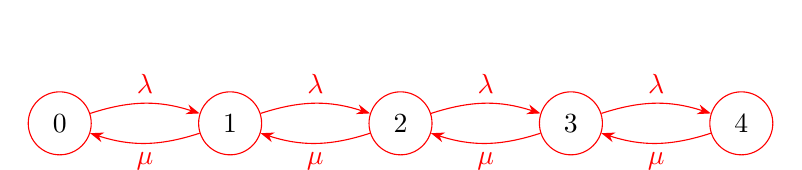
\begin{tikzpicture}[
  state/.style={circle,draw=red,minimum size=8mm},
  >=Stealth,
  node distance=1.35cm
]
  \node[state] (s0) {$0$};
  \node[state,right=of s0] (s1) {$1$};
  \node[state,right=of s1] (s2) {$2$};
  \node[state,right=of s2] (s3) {$3$};
  \node[state,right=of s3] (s4) {$4$};
  \foreach \a/\b in {s0/s1,s1/s2,s2/s3,s3/s4}{
    \draw[->,red,bend left=18] (\a) to node[above,text=red] {$\lambda$} (\b);
    \draw[->,red,bend left=18] (\b) to node[below,text=red] {$\mu$} (\a);
  }
\end{tikzpicture}
\end{center}
Arrivals in state 4 are rejected and therefore do not change the state.

\textbf{(b)} Local balance gives
\[
\lambda\pi_n=\mu\pi_{n+1},
\qquad n=0,1,2,3.
\]
With $\rho=\lambda/\mu=1/2$, we have $\pi_n=\rho^n\pi_0$. Normalization gives
\[
1=\pi_0\sum_{n=0}^{4}\left(\frac12\right)^n
=\pi_0\frac{31}{16}.
\]
Therefore,
\answerbox{
(\pi_0,\pi_1,\pi_2,\pi_3,\pi_4)
=\left(\frac{16}{31},\frac8{31},\frac4{31},\frac2{31},\frac1{31}\right)
}

\textbf{(c)} The utilization is the probability that the server is busy:
\[
1-\pi_0=\frac{15}{31}\approx0.4839.
\]

\textbf{(d)} By PASTA (Poisson Arrivals See Time Averages), an arrival sees a full
system with the steady-state probability $\pi_4$. Hence
\[
P_{\mathrm{loss}}=\pi_4=\frac1{31}\approx0.0323.
\]

\textbf{(e)}
\[
\E[N]=\sum_{n=0}^{4}n\pi_n=\frac{26}{31}\approx0.8387.
\]

\textbf{(f)} The effective arrival rate of admitted jobs is
\[
\lambda_e=\lambda(1-\pi_4)=2\left(1-\frac1{31}\right)
=\frac{60}{31}.
\]
By Little's Law for admitted jobs,
\[
\E[T]=\frac{\E[N]}{\lambda_e}
=\frac{26/31}{60/31}=\frac{13}{30}\approx0.4333\text{ seconds}.
\]

\textbf{(g)} For an $M/M/1/K$ queue,
\[
\pi_K=\frac{\rho^K}{\sum_{n=0}^{K}\rho^n}.
\]
If capacity is doubled to $K=8$, $\rho=1/2$ and
\[
P_{\mathrm{loss}}=\frac{(1/2)^8}{\sum_{n=0}^{8}(1/2)^n}
=\frac1{511}\approx0.00196.
\]
If speed is doubled to $\mu=8$, then $K=4$, $\rho=1/4$, and
\[
P_{\mathrm{loss}}=\frac{(1/4)^4}{\sum_{n=0}^{4}(1/4)^n}
=\frac1{341}\approx0.00293.
\]
\answerboxtext{\textbf{(g)} Doubling system capacity is better:
$1/511<1/341$.}

\textbf{(h)} If capacity is doubled, then $K=8$ and $\rho=3/4$:
\[
P_{\mathrm{loss}}
=\frac{(3/4)^8}{\sum_{n=0}^{8}(3/4)^n}
=\frac{6561}{242461}\approx0.0271.
\]
If speed is doubled, then $K=4$ and $\rho=3/8$:
\[
P_{\mathrm{loss}}
=\frac{(3/8)^4}{\sum_{n=0}^{4}(3/8)^n}
=\frac{81}{6505}\approx0.0125.
\]
\answerboxtext{\textbf{(h)} Doubling CPU speed is better:
$81/6505<6561/242461$.}

\textbf{(i)} When $\rho=1/2$, the system is lightly loaded and seldom fills, so
four extra buffer slots nearly eliminate an already rare rejection event. When
$\rho=3/4$, sustained service congestion is the main issue. Extra buffer space only
stores waiting jobs, while faster service directly removes the bottleneck and reduces
the probability of reaching capacity.
\end{solution}
\end{examquestion}

% -----------------------------------------------------------------------------
\begin{examquestion}{6}{10}
Suppose your computer center currently consists of a single server of speed $\mu$.
Jobs arrive according to a Poisson process with rate $\lambda$, and their service times
are exponentially distributed.

Suppose the current response time is considered intolerable by the users. A second,
faster server, running at speed $\alpha\mu$ (for $\alpha>1$), is purchased and added
to the system. With the second server, the system becomes a variant of the $M/M/2$
queue where the service rates of the two processors are not identical. Denote the
service rate of the first processor by $\mu_1=\mu$ and the service rate of the second
processor by $\mu_2=\alpha\mu$, where $\mu_1<\mu_2$. In such a system, when both
servers are idle, the faster server is scheduled for service before the slower one.
Define the utilization, $\rho<1$, by
\[
\rho=\frac{\lambda}{\mu_1+\mu_2}.
\]

Suppose the mean response time is given by
\[
\E[T]=\frac{1}{\lambda A(1-\rho)^2},
\]
where
\[
A=\frac{\mu_1\mu_2(1+2\rho)}{\lambda(\lambda+\mu_1)}
+\frac{1}{1-\rho}.
\]
Determine the mean number of jobs $\E[N]$ in the system. You do not need to simplify
your answer.

\begin{solution}
By Little's Law, $\E[N]=\lambda\E[T]$. Therefore,
\[
\E[N]
=\lambda\frac{1}{\lambda A(1-\rho)^2}
=\frac{1}{A(1-\rho)^2}.
\]
Hence,
\answerbox{\E[N]=\frac{1}{A(1-\rho)^2}}
where
\[
A=\frac{\mu_1\mu_2(1+2\rho)}{\lambda(\lambda+\mu_1)}
+\frac{1}{1-\rho},
\qquad
\rho=\frac{\lambda}{\mu_1+\mu_2}<1.
\]
\end{solution}
\end{examquestion}

% -----------------------------------------------------------------------------
\begin{examquestion}{7}{10}
In Question 6, a hotshot consultant walks in and makes the radical proposal of
disconnecting the original server entirely (i.e., simply letting the faster server run
by itself). Clearly this makes sense with respect to power, but the consultant claims
this is also a win for $\E[N]$. For a consulting fee of \$400/hr, what is the
consultant thinking? Come up with an instance, with specific values for $\lambda$,
$\mu_2$, and $\mu_1$ for which the consultant is right. Also, explain intuitively what
is happening. [If you find this problem interesting, you can think about a general
criterion under which the consultant would be right. Throwing away servers is fun!]

\begin{solution}
Choose
\answerbox{
\lambda=5,
\qquad
\mu_1=1,
\qquad
\mu_2=10
}
Both systems are stable because $5<1+10$ and $5<10$. For the two-server system,
\[
\rho=\frac{5}{1+10}=\frac5{11},
\]
and, using the formula printed in Question 6,
\[
\begin{aligned}
A
&=\frac{(1)(10)(1+2\cdot5/11)}{5(5+1)}+\frac{1}{1-5/11}\\
&=\frac7{11}+\frac{11}{6}=\frac{163}{66}.
\end{aligned}
\]
Therefore,
\[
\E[N]_{\text{two-server}}
=\frac{1}{(163/66)(1-5/11)^2}
=\frac{1331}{978}
\approx1.3609.
\]

If the slower server is disconnected, the system becomes an $M/M/1$ queue with
arrival rate 5 and service rate 10. Its mean number of jobs is
\[
\E[N]_{\text{fast-only}}
=\frac{\lambda}{\mu_2-\lambda}
=\frac{5}{10-5}=1.
\]
Thus,
\answerbox{
\E[N]_{\text{fast-only}}=1
<\frac{1331}{978}
=\E[N]_{\text{two-server}}
}
Disconnecting the slower server reduces the mean number of jobs in this instance.

\textbf{Intuition:} Under the fast-server-first rule, an arrival that finds the fast
server busy but the slow server idle is sent directly to the slow server. With the
large speed difference here, that job may spend much longer in slow service than it
would spend waiting briefly for the fast server and then receiving fast service. The
fast server alone has utilization $5/10=1/2$, so it has enough spare capacity for this
waiting-for-fast strategy to reduce $\E[N]$.
\end{solution}
\end{examquestion}

\label{LastPage}
\thispagestyle{lastpage}

\end{document}
